%\begin{figure}[!htpb]
%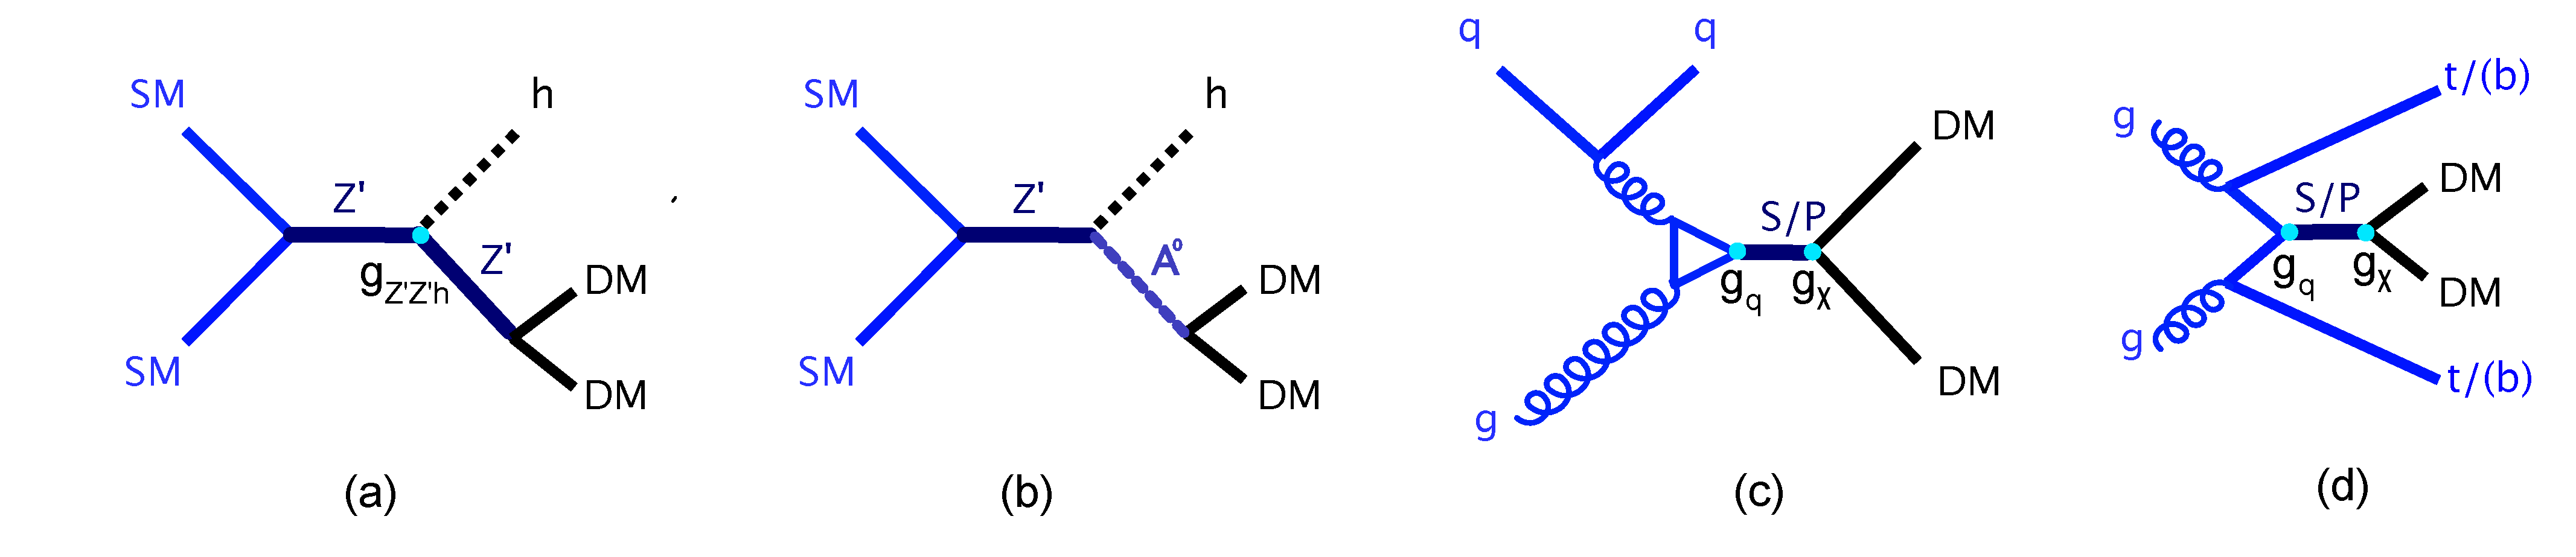
\includegraphics[width=\textwidth]{figures/feynman_1}
%\caption{

(\textit{a}) Example of a process including baryonic coupling between a vector mediator $Z'$ and an SM Higgs boson. The $Z'$--Higgs coupling is denoted \ghZprimeZprime. 
(\textit{b}) Example of a process from a \textit{U}(1) $Z'$ boson embedded in a 2HDM, where a vector $Z'$ decays to a pseudoscalar $A^0$ that in turn decays to DM particles. 
(\textit{c,d}) Examples of a simplified model process where the interaction is mediated by an intermediate scalar or pseudoscalar particle. In panel \textit{c}, the SM--scalar interaction proceeds through a gluon loop \cite{Haisch:2013ata}, whereas in panel \textit{d}, the pseudo(scalar) is produced in association with a pair of heavy-flavor quarks. The coupling constants that are prefactors to the Yukawa couplings in the model are denoted \gq for the mediator--quark--quark vertex and \gdm for the mediator--DM vertex. 
Abbreviations:\ $A^0/a$, pseudoscalar bosons; $b$, bottom quark; DM, dark matter;  $g$, gluon; $h$, SM Higgs boson; $S$, heavy scalar boson; SM, Standard Model; $t$, top quark; $Z'$, vector mediator; 2HDM, two--Higgs doublet model. 

%}
%\label{fig:feynman_1}
%\end{figure}